\begin{frame}{Scientific context}
	\begin{minipage}{0.78\linewidth}
		\textbf{Context :} Create real-time digital twins of an organ (e.g. liver).
	\end{minipage}
	\begin{minipage}{0.18\linewidth}
		\vspace{-20pt}
		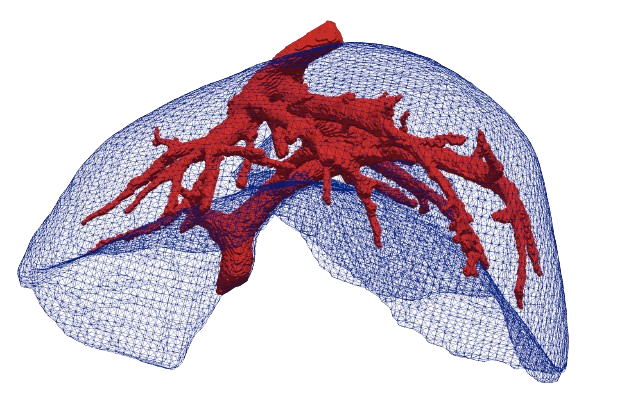
\includegraphics[width=0.95\linewidth]{images/intro/liver.png}
	\end{minipage}
	
	\vspace{1pt}
	\textbf{Objective :} Develop an hybrid \fcolorbox{red}{white}{finite element} / \fcolorbox{orange}{white}{neural network} method.
	
	\vspace{1pt}
	\small
	\hspace{130pt} \begin{minipage}{0.14\linewidth}
		\textcolor{red}{accurate}
	\end{minipage} \hspace{8pt} \begin{minipage}{0.3\linewidth}
		\textcolor{orange}{quick + parameterized}
	\end{minipage}

	\normalsize
	\vspace{5pt}
	\textbf{Parametric linear elliptic PDE :}
	For one or several  $\bm{\mu}\in \mathcal{M}$, find $u: \Omega\to \mathbb{R}$ such that
	\begin{equation}
		\label{eq:ob_pde}
		\mathcal{L}\big(u;\bm{x},\bm{\mu}\big) = f(\bm{x},\bm{\mu}),
		\tag{$\mathcal{P}$}
	\end{equation}
	where $\mathcal{L}$ is the parametric differential operator defined  by
	\begin{equation*}
		\mathcal{L}(\cdot;\bm{x},\bm{\mu}) : u \mapsto R(\bm{x},\bm{\mu}) u + C(\bm{\mu}) \cdot \nabla u - \frac{1}{\text{Pe}} \nabla \cdot (D(\bm{x},\bm{\mu}) \nabla u),
	\end{equation*}
	and some Dirichlet, Neumann or Robin BC (which can also depend on $\bm{\mu}$).
	
	\footnotesize
	\begin{table}[ht!]
		\centering
		\begin{tabular}{c|c}
			$\Omega$ & Spatial domain \\
			$d$ & Spatial dimension \\
			$\bm{x}=(x_1,\dots,x_d)$ & Spatial coordinates \\
			\hline
			$\mathcal{M}$ & Parameter space \\
			$p$ & Number of parameters \\
			$\bm{\mu}=(\mu_1,\ldots,\mu_p)$ & Parameter vector \\
		\end{tabular} \hspace{10pt}
		\begin{tabular}{c|c}
			$f$ & Right-hand side \\
			$R$ & Reaction coefficient \\
			$C$ & Convection coefficient \\
			$D$ & Diffusion matrix \\
			Pe & Péclet number \\
		\end{tabular}
	\end{table}
\end{frame}

\begin{frame}{Pipeline of the Enriched FEM}
	\begin{figure}[!ht]
		\centering
		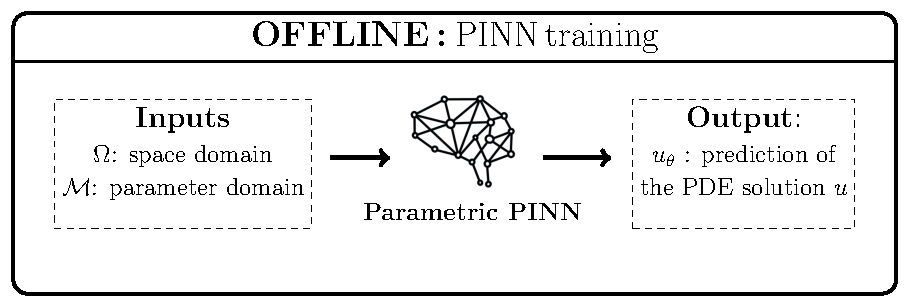
\includegraphics[width=0.7\linewidth]{images/intro/pipeline/offline_v2.pdf}

		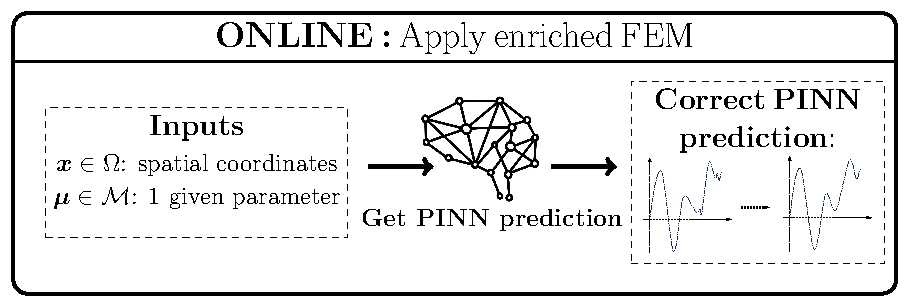
\includegraphics[width=0.7\linewidth]{images/intro/pipeline/online_v2.pdf}
	\end{figure}

	\textbf{Correction :} Enriched continuous Lagrange finite element approximation spaces
	using the PINN prediction.
\end{frame}

\begin{frame}{Physics-Informed Neural Networks}
	\textbf{Standard PINNs\footcite{RAISSI2019686} (Weak BC) :} Find the optimal weights $\theta^\star$ that satisfy
	\begin{equation}
		\label{eq:opt_pb}
		\theta^\star = \argmin_{\theta}	\big( \omega_r \; J_r(\theta) + \omega_b \; J_b(\theta) \big),
		\tag{$\mathcal{P}_\theta$}
	\end{equation}
	with the residual loss function and the boundary loss function defined by
	\begin{equation*}
		J_r(\theta) =
		\int_{\mathcal{M}}\int_{\Omega}
		\big| \mathcal{L}\big(u_\theta(\bm{x},\bm{\mu});\bm{x},\bm{\mu}\big)-f(\bm{x},\bm{\mu}) \big|^2 d\bm{x} d\bm{\mu},
	\end{equation*}
	\begin{equation*}
		J_b(\theta) =
		\int_{\mathcal{M}}\int_{\partial \Omega} \big| u_\theta(\bm{x},\bm{\mu}) - g(\bm{x},\bm{\mu}) \big|^2 d\bm{x} d\bm{\mu},
	\end{equation*}
	where $u_\theta$ is a neural network, $g=0$ is the Dirichlet BC. In \eqref{eq:opt_pb}, the weights $\omega_r$ and $\omega_b$ (hyperparameters) are used to balance the different terms of the loss function.

	\vspace{5pt}
	\textbf{Monte-Carlo method :} Discretize the cost functions by random process.
	\vspace{15pt}
\end{frame}

\begin{frame}[noframenumbering]{Physics-Informed Neural Networks}
	\textbf{\textcolor{red}{Improved PINNs\footcite{LagLikFot1998,FraMicNav2024} (Strong BC)} :} Find the optimal weights $\theta^\star$ that satisfy
	\begin{equation*}
		% \label{eq:opt_pb_nobc}
		\theta^\star = \argmin_{\theta}	\big( \omega_r \; J_r(\theta) + \Ccancel[red]{\omega_b \; J_b(\theta)} \big),%\tag{$\mathcal{P}_\theta$}
	\end{equation*}
	with $\omega_r=1$ and the residual loss function defined by
	\begin{equation*}
		J_r(\theta) =
		\int_{\mathcal{M}}\int_{\Omega}
		\big| \mathcal{L}\big(u_\theta(\bm{x},\bm{\mu});\bm{x},\bm{\mu}\big)-f(\bm{x},\bm{\mu}) \big|^2 d\bm{x} d\bm{\mu},
	\end{equation*}
	\begin{minipage}{0.75\linewidth}
		where $u_\theta$ is a neural network defined by
		\begin{equation*}
			\textcolor{red}{u_{\theta}(\bm{x},\bm{\mu}) = \varphi(\bm{x}) w_{\theta}(\bm{x},\bm{\mu}) + g(\bm{x},\bm{\mu}),}
		\end{equation*}
		with $\varphi$ a level-set function, $w_\theta$ a NN and $g=0$ the Dirichlet BC. 
	\end{minipage}
	\begin{minipage}{0.23\linewidth}
		\vspace{-15pt}
		\hspace{-23pt}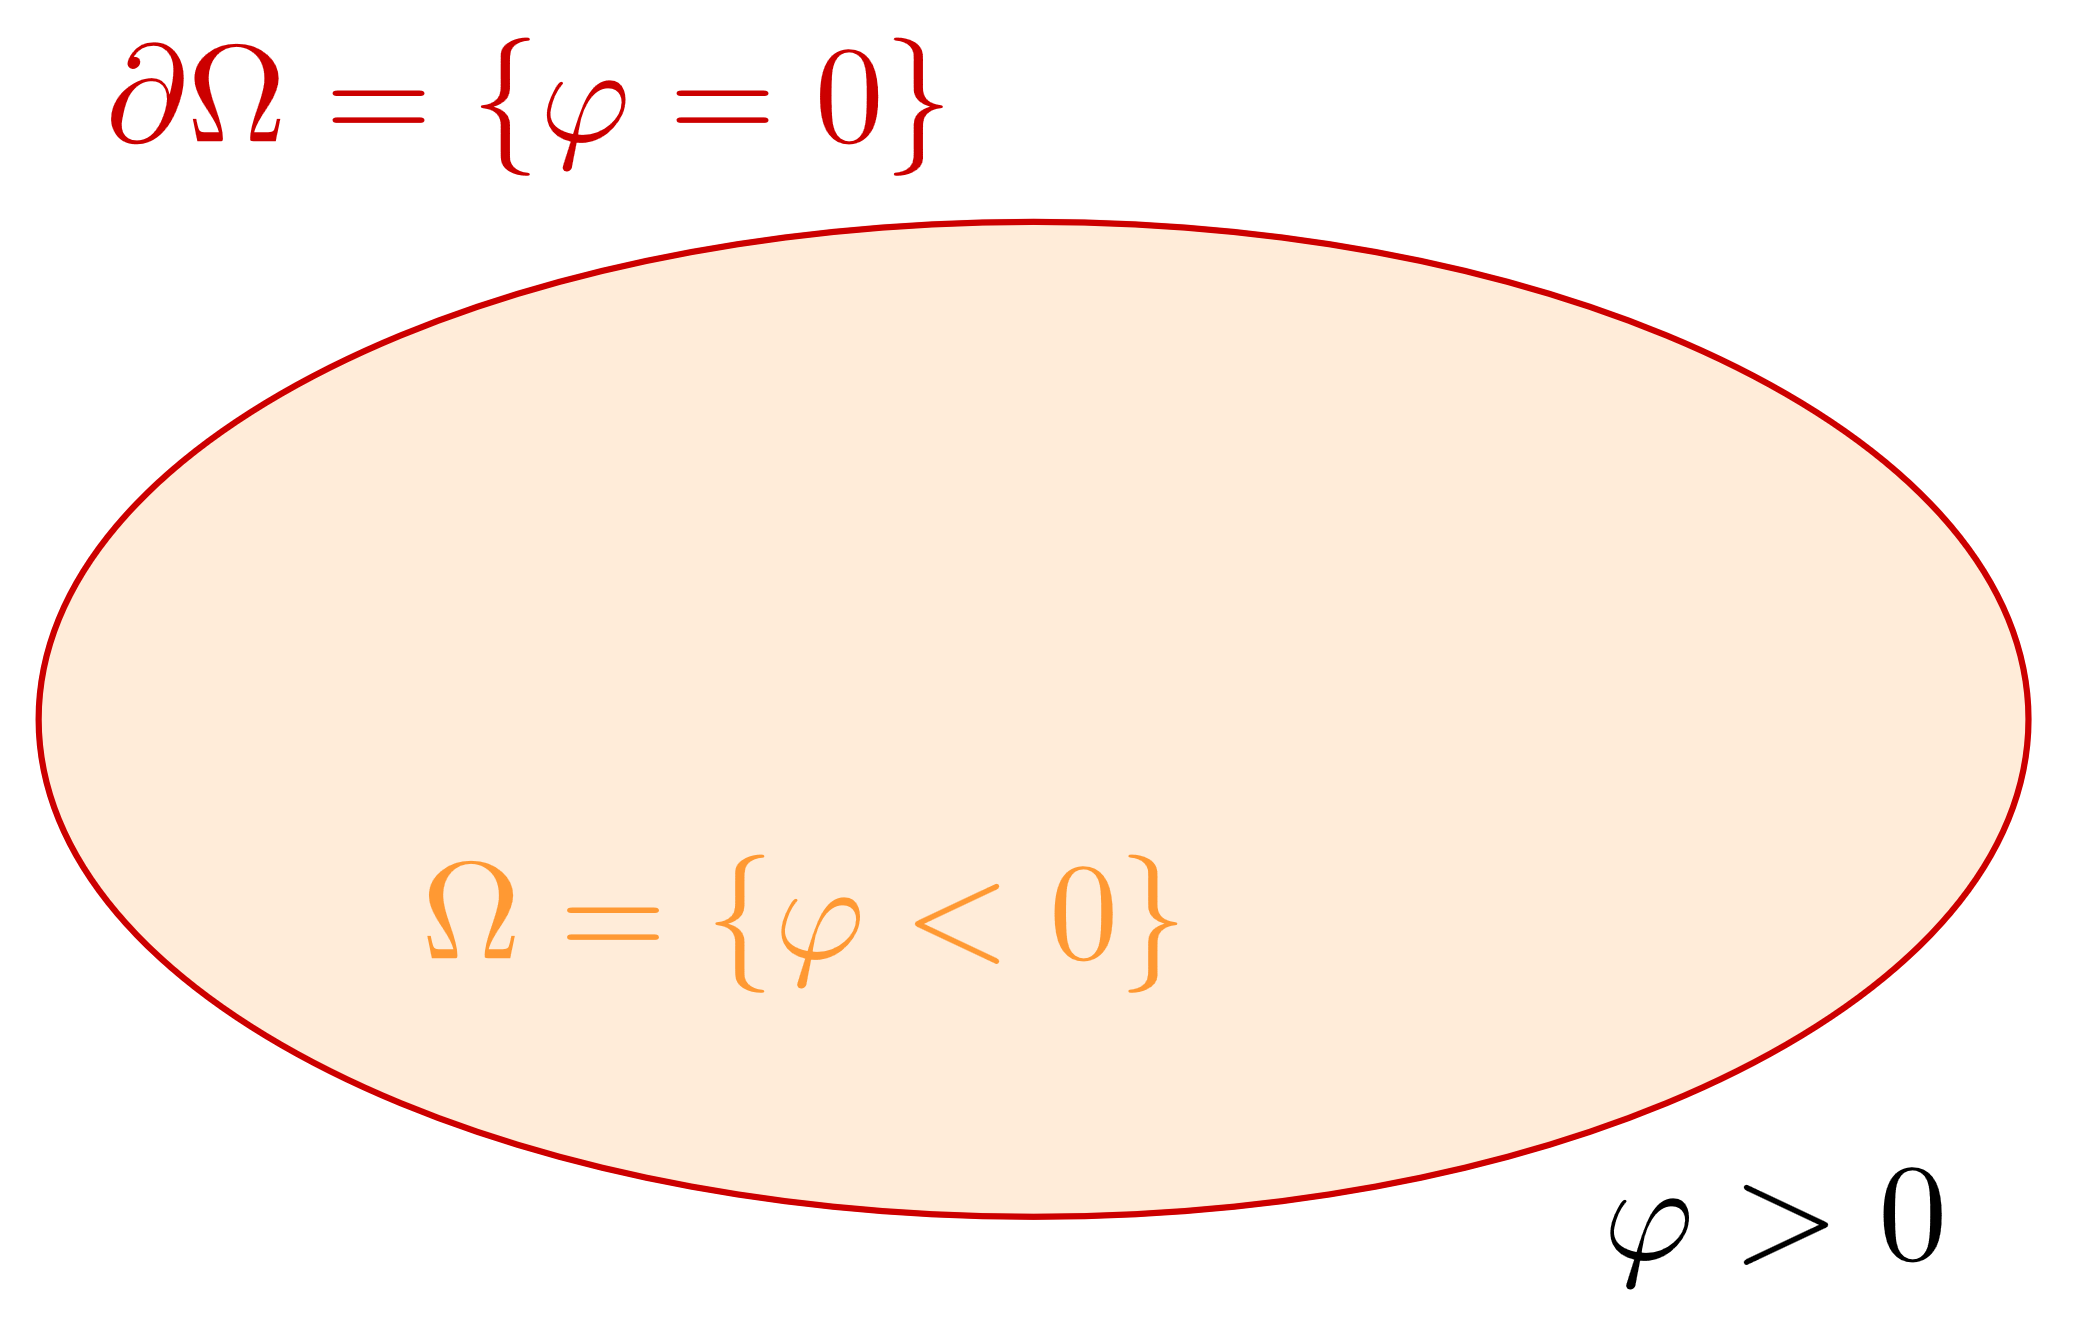
\includegraphics[width=1.3\linewidth]{images/intro/levelset.png}
	\end{minipage}

	Thus, the Dirichlet BC is imposed exactly in the PINN : \textcolor{red}{$u_{\theta} = g$ on $\partial \Omega$}.

	\vspace{5pt}
	\textbf{Monte-Carlo method :} Discretize the residual cost function by random process.
	\vspace{15pt}
\end{frame}


\begin{frame}{Finite Element Method\footcite{Ern2004TheoryAP}}	
	\textbf{Variational Problem :} 
	\begin{equation}
		\label{eq:weakform}
		\text{Find } u_h\in V_h^0 \text{such that}, \forall v_h\in V_h^0, a(u_h,v_h)=l(v_h),
		\tag{$\mathcal{P}_h$}
	\end{equation}
	\vspace{1pt}
	with $h$ the characteristic mesh size, $a$ and $l$ the bilinear and linear forms given by
	\vspace{-3pt}
	\begin{equation*}
		a(u_h,v_h)=
		\frac{1}{\text{Pe}} \int_{\Omega}D \nabla u_h \cdot  \nabla v_h+
		\int_{\Omega} R \, u_h \, v_h  +
		\int_{\Omega} v_h \, C \cdot \nabla u_h, \quad l(v_h)=\int_{\Omega} f \, v_h,
	\end{equation*}

	\begin{minipage}[t]{0.7\linewidth}
		\vspace{-3pt}
		and $V_h$ the finite element space of dimension $N_h$ defined by
		\vspace{-3pt}
		\begin{equation*}
			% \label{eq:Vh}
			V_h = \left\{v_h\in C^0(\Omega),\; \forall K\in \mathcal{T}_h,\; v_h\vert_{K}\in\mathbb{P}_k,v_h\vert_{\partial\Omega}=0\right\},
		\end{equation*}

		\vspace{-3pt}
		where $\mathbb{P}_k$ is the space of polynomials of degree at most $k$.

		\vspace{10pt}
		\textbf{Linear system :} Let $(\phi_1,\dots,\phi_{N_h})$ a basis of $V_h$.
	\end{minipage} \qquad \begin{minipage}[t][][b]{0.2\linewidth}
		% \vspace{-5pt}
		\centering
		\pgfimage[width=0.9\linewidth]{images/intro/FEM_triangle_mesh.png}
		
		\footnotesize
		$\mathcal{T}_h = \left\{K_1,\dots,K_{N_e}\right\}$
		
		\tiny
		($N_e$ : number of elements)
	\end{minipage}

	\vspace{-5pt}
	Find $U\in\mathbb{R}^{N_h}$ such that \hspace{40pt} $AU=b$

	with 
	\begin{equation*}
		A=\big(a(\phi_i,\phi_j)\big)_{1\le i,j\le N_h} \quad \text{and} \quad b=\big(l(\phi_j)\big)_{1\le j\le N_h}.
	\end{equation*}
	\vspace{-3pt}
\end{frame}